\section{Pruning two families of pairs}\label{sec:pruning}

We now prove a deletion bound for two families of ordered pairs.  The bound
charges the deleted members to two sets of pairs: one determined by the
original conflicts, and the other consisting of points left uncovered after
deletion.  This dependence on the surviving families will be essential in
Section~\ref{sec:incompatibility}.  The result holds for every finite binary
relation; no orientation assumption is needed.

\begin{lemma}[Pruning]\label{lem:pruning}
Let $X$ be a finite set with a binary relation denoted by $\to$, and let
$\mathcal R,\mathcal C\subseteq X\times X$ be two families, regarded as
separate copies even when their coordinates agree.  Say that
$(p,j)\in\mathcal R$ and $(i,s)\in\mathcal C$ \emph{conflict} if
\[
 p\to i\qquad\text{and}\qquad s\to j.
\]
Define
\begin{align*}
 Z&=\{(i,j):\text{some }(p,j)\in\mathcal R
       \text{ conflicts with some }(i,s)\in\mathcal C\},\\
 H&=\{(p,s):\text{some }(p,j)\in\mathcal R
       \text{ conflicts with some }(i,s)\in\mathcal C\}.
\end{align*}
A point $(i,j)$ is \emph{covered} by a member $(p,j)\in\mathcal R$ when
$p\to i$, and by a member $(i,s)\in\mathcal C$ when $s\to j$.
These are the only ways a member covers a point.

There are subfamilies $\mathcal R'\subseteq\mathcal R$ and
$\mathcal C'\subseteq\mathcal C$ with no conflicts between them such that
every initially conflict-free member is retained and
\begin{equation}\label{eq:pruning-bound}
 \abs{\mathcal R\setminus\mathcal R'}+
 \abs{\mathcal C\setminus\mathcal C'}
 \leq \abs H+
 \abs{\{z\in Z:z\text{ is covered by no member of }
                    \mathcal R'\cup\mathcal C'\}}.
\end{equation}
The two sides are counted separately throughout.
\end{lemma}

The proof will bound a matching in an augmented bipartite graph by using
matrix ranks.  We first record the elementary rank fact that makes the
argument work.  For finite index sets $I,J$, a matrix supported on
$T\subseteq I\times J$ means a real matrix whose entries outside $T$ are
zero; entries in $T$ are allowed to vanish.

\begin{lemma}[Kernels at maximum support rank]\label{lem:kernel-support}
Let $T\subseteq I\times J$, where $I$ and $J$ are finite.  Suppose that
$D:\R^J\to\R^I$ has maximum rank among all real matrices supported on $T$.
Then, for every $x\in\ker D$, every $y\in\ker D^{\mathsf T}$, and every
$(s,j)\in T$, one has $x_jy_s=0$.
\end{lemma}

\begin{proof}
Suppose instead that $x_jy_s\ne0$.  For a nonzero real $\tau$, the matrix
$D_\tau=D+\tau e_s e_j^{\mathsf T}$ is still supported on $T$, and
\[
 D_\tau x=\tau x_j e_s.
\]
Thus $e_s\in\im D_\tau$.  Moreover, for every $w\in\R^J$,
\[
 Dw=D_\tau w-\tau w_j e_s\in\im D_\tau,
\]
so the entire old image $\im D$ is contained in $\im D_\tau$.
On the other hand, $y$ annihilates $\im D$ and $y_s\ne0$, so
$e_s\notin\im D$.  Therefore $\rank D_\tau>\rank D$, a contradiction.
\end{proof}

\begin{proof}[Proof of Lemma~\ref{lem:pruning}]
If there are no conflicts, retain every member; then $Z=H=\varnothing$
and the assertion is immediate.  In what follows, all vector spaces have
their usual coordinate bases.  Empty minors have determinant $1$, so the
rank arguments also apply when a matching or an index set is empty.

\medskip\noindent
\emph{The augmented graph and the required matching bound.}
Form a bipartite graph $\Gamma$ with parts
\[
 \mathcal V_L=\mathcal R\sqcup Z_L,
 \qquad
 \mathcal V_R=\mathcal C\sqcup Z_R,
\]
where $Z_L$ and $Z_R$ are separate copies of $Z$, disjoint also from the
two original families.  Join conflicting original members.  Also join
each original member to the opposite copy of every point of $Z$ that it
covers.  There are no edges between $Z_L$ and $Z_R$.
Figure~\ref{fig:pruning} displays the three edges forced by one conflict.

\begin{figure}[!ht]
 \centering
 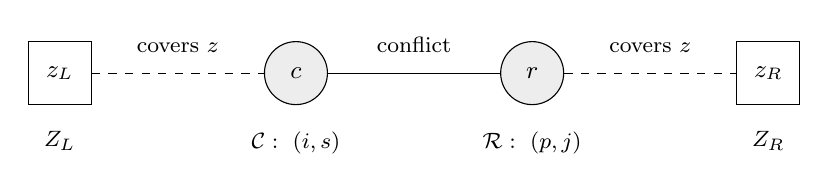
\begin{tikzpicture}[
  every node/.style={font=\small},
  original/.style={circle,draw,fill=black!7,minimum size=8mm,inner sep=1pt},
  copy/.style={rectangle,draw,minimum size=8mm,inner sep=3pt},
  edge label/.style={font=\footnotesize,above=4pt},
  family label/.style={font=\footnotesize,below=6pt}
]
 \node[copy] (zl) at (0,0) {$z_L$};
 \node[original] (c) at (3,0) {$c$};
 \node[original] (r) at (6,0) {$r$};
 \node[copy] (zr) at (9,0) {$z_R$};
 \draw[dashed] (zl) -- node[edge label] {covers $z$} (c);
 \draw (c) -- node[edge label] {conflict} (r);
 \draw[dashed] (r) -- node[edge label] {covers $z$} (zr);
 \node[family label] at (zl.south) {$Z_L$};
 \node[family label] at (c.south) {$\mathcal C:\ (i,s)$};
 \node[family label] at (r.south) {$\mathcal R:\ (p,j)$};
 \node[family label] at (zr.south) {$Z_R$};
\end{tikzpicture}

 \caption{A conflict between $r=(p,j)$ and $c=(i,s)$ forces this path,
 where $z=(i,j)\in Z$.  The copies $z_L$ and $z_R$ are distinct vertices.
 The vertices alternate between the two sides of the bipartition.
 Different conflicts can share vertices and edges; the full augmented
 graph need not be a disjoint union of such paths.}
 \label{fig:pruning}
\end{figure}

An initially conflict-free member is isolated in $\Gamma$.
Indeed, if $(p,j)\in\mathcal R$ covered $(i,j)\in Z$, an original
conflict witnessing $(i,j)\in Z$ would supply a member
$(i,s)\in\mathcal C$ with $s\to j$.  This member would conflict with
$(p,j)$.  The same argument with the sides exchanged applies to
$\mathcal C$.

It suffices to find a vertex cover $K$ of $\Gamma$ of size at most
$\abs Z+\abs H$, omitting isolated vertices.  Delete precisely its
original members.  No conflict then survives.  If $q$ points of $Z$ are
uncovered by the surviving members, each of the other $\abs Z-q$ points
has a surviving member adjacent to one of its two copies.  That copy
must lie in $K$.  Distinct points require distinct new vertices, whence
\begin{equation}\label{eq:cover-charge}
 \abs{K\cap(\mathcal R\sqcup\mathcal C)}
 \leq \abs K-(\abs Z-q)\leq\abs H+q.
\end{equation}
Thus the cover gives exactly~\eqref{eq:pruning-bound} and retains every
initially conflict-free member.

We will obtain this cover by proving that a maximum matching in $\Gamma$
has size at most $\abs Z+\abs H$ and then giving the usual alternating-path
construction of the cover.  Choose a maximum matching $\mathcal M$ with
the fewest edges between original members.  Write $k$ for the number of
these edges, and let $\alpha$ and $\beta$ be its edges in
$\mathcal R\times Z_R$ and $Z_L\times\mathcal C$, respectively.  Put
\[
 \ell=\abs\alpha,\qquad t=\abs\beta,
 \qquad\abs{\mathcal M}=k+\ell+t.
\]

Each of $\alpha$ and $\beta$ is a maximum matching in its own subgraph.
For example, if the $\mathcal R$--$Z_R$ subgraph had a larger matching,
its symmetric difference with $\alpha$ would contain an
$\alpha$-augmenting path, starting at an $\alpha$-unmatched member of
$\mathcal R$ and ending at an $\alpha$-unmatched vertex of $Z_R$.
The latter vertex is unmatched in $\mathcal M$, and every internal vertex
of the path is matched by $\alpha$.  If the starting member is unmatched
in $\mathcal M$, augmenting gives a larger matching in $\Gamma$.
Otherwise it lies on an original--original edge of $\mathcal M$;
remove that edge and augment along the path.  This preserves the total
size and reduces $k$.  Both conclusions contradict the choice of
$\mathcal M$.  The proof for $\beta$ is identical with the sides
exchanged.  Denote by $R_\alpha\subseteq\mathcal R$ and
$C_\beta\subseteq\mathcal C$ the original vertices matched by these
two matchings.

\medskip\noindent
\emph{Four maps and a simultaneous choice of coefficients.}
To bound $k+\ell+t$, we encode the two maximum matchings by matrix ranks.
For each arrow $x\to y$, introduce independent variables $a_{xy}$ and
$b_{xy}$, with the two arrays independent of one another.  Set both
entries to zero when $x\not\to y$.  We shall choose real values for all
the variables shortly.  For any real assignment, define four maps by
\[
 \begin{array}{ccc}
 \R^{\mathcal R}&\xrightarrow{\ L\ }&\R^Z\\[3pt]
 {\scriptstyle B}\big\downarrow&&\big\downarrow{\scriptstyle N}\\[3pt]
 \R^H&\xrightarrow{\ A\ }&\R^{\mathcal C}
 \end{array}
\]
with entries
\begin{equation}\label{eq:pruning-maps}
 \begin{aligned}
 L_{(i,j),(p,j)}&=a_{pi},&
 N_{(i,s),(i,j)}&=b_{sj},\\
 B_{(p,s),(p,j)}&=b_{sj},&
 A_{(i,s),(p,s)}&=a_{pi}.
 \end{aligned}
\end{equation}
The row and column indices in each formula range over its indicated
coordinate sets, and every entry not of a listed form is zero.
The maps $L,A$ change the first coordinate forward along $p\to i$;
$N,B$ change the second coordinate backward from $j$ to $s$ along $s\to j$.
For a conflict, the two routes from $(p,j)$ to $(i,s)$ change the
coordinates in opposite orders, through $(i,j)\in Z$ or $(p,s)\in H$.
For a fixed column $(p,j)\in\mathcal R$ and row
$(i,s)\in\mathcal C$, the only possible intermediate index in $NL$ is
$(i,j)$, and the only possible one in $AB$ is $(p,s)$.  If the two
endpoints conflict, these indices belong to $Z$ and $H$, respectively,
and both products have entry $a_{pi}b_{sj}$.  If they do not conflict,
at least one factor is zero in both products.  Hence
\begin{equation}\label{eq:pruning-commute}
 NL=AB.
\end{equation}

We seek an assignment for which
\[
 \rank L=\ell,\qquad \rank N=t,\qquad \dim\ker A\geq k.
\]
These three conditions give the desired matching bound. Indeed,
rank--nullity and $NL=AB$ would give
\begin{align}
 \abs H
 &=\dim\ker A+\rank A\notag\\
 &\geq k+\rank A
 \geq k+\rank(NL)\notag\\
 &\geq k+\ell+t-\abs Z.
 \label{eq:pruning-rank-bound}
\end{align}
The last inequality follows by restricting $N$ to $\im L$:
\[
 \rank(NL)
 =\dim\im L-\dim(\im L\cap\ker N)
 \geq\ell-(\abs Z-t).
\]
The first two rank conditions will come from $\alpha$ and $\beta$.
For the third, we will lift the $k$ original left endpoints to vectors
$u^r\in\ker L$ and show that their images $Bu^r$ are independent.
The identity $AB=NL$ places these images in $\ker A$.

Our choice of coefficients uses the correspondence between generic matrix
rank and maximum matching size~\cite[Section~5, Theorem~1]{Edmonds1967}.
We apply the determinant argument within coordinate blocks and verify that
all required minors can be nonzero at the same assignment.
We choose the coefficients so that $\rank L=\ell$, with its
$R_\alpha$ columns a basis of $\im L$, and
$\rank N^{\mathsf T}=t$, with its $C_\beta$ columns a basis of
$\im N^{\mathsf T}$.  To justify this choice, a nonzero minor of $L$
requires a matching between its column and row indices: a nonzero term
in its determinant supplies the matching.  Since $\alpha$ is maximum,
$\rank L\leq\ell$ for every coefficient assignment.  The square minor
using precisely the endpoints of $\alpha$ is, up to row and column
ordering, block diagonal by the second coordinate $j$.  In each block
all allowed entries are distinct variables $a_{pi}$.  The matching
gives a determinant monomial that cannot cancel, because different
permutations use different sets of these variables.  Each block
determinant is therefore a nonzero polynomial, and so is their product.
Variables may occur in more than one block, but a product of nonzero
polynomials remains nonzero.  This proves the required independence
when that minor does not vanish.  For $N^{\mathsf T}$ the same argument
uses blocks with the first coordinate $i$ fixed and distinct variables
$b_{sj}$ within each block.

One additional finite collection of rank conditions will be needed.
For every arrow $p\to i$, define
\[
 J_p=\{j:(p,j)\in\mathcal R\},\qquad
 S_i=\{s:(i,s)\in\mathcal C\},\qquad
 D^{p,i}=(b_{sj})_{s\in S_i,\ j\in J_p}.
\]
We require $D^{p,i}$ to have maximum rank among all matrices supported
on
\[
 T^{p,i}=\{(s,j)\in S_i\times J_p:s\to j\}.
\]
These matrices will let Lemma~\ref{lem:kernel-support} compare restrictions
of vectors in $\ker B$ and $\ker N^{\mathsf T}$.
The allowed entries of each individual $D^{p,i}$ are independent
variables.  A minor attaining its maximum possible rank at some
assignment is therefore a nonzero polynomial in the $b$ variables.
Choose one such minor for each arrow, taking the empty minor when the
maximum rank is zero.  Multiply these finitely many polynomials with
the two matching minors just described.  The product is nonzero in the
polynomial ring generated by all $a$ and $b$ variables, even though
variables are shared between different matrices.  A nonzero real
polynomial is nonzero at some real assignment, as follows by induction
on its number of variables.  Fix such an assignment once and for all.
It gives these support ranks and the two basis properties simultaneously.

For every edge $(r,c)$ of $\mathcal M$ between original members, the
basis properties now give vectors
\begin{equation}\label{eq:pruning-lifts}
 \begin{aligned}
 u^r&=e_r+\sum_{a\in R_\alpha}\lambda_a^r e_a
                 \in\ker L,\\
 v^c&=e_c+\sum_{b\in C_\beta}\mu_b^c e_b
                 \in\ker N^{\mathsf T}.
 \end{aligned}
\end{equation}
The original--original endpoints are disjoint from $R_\alpha$ and
$C_\beta$, respectively.  In particular, the $u^r$ restrict to distinct
unit vectors on the $k$ original left endpoints, and $v^c_c=1$.

\medskip\noindent
\emph{The kernel restriction and the matching bound.}
It remains to show that the $k$ lifts just constructed give independent
vectors $Bu^r$. The key assertion, at our fixed coefficient assignment, is
\begin{equation}\label{eq:conflict-kernel}
 u_{pj}v_{is}=0
 \quad\text{for every conflict }((p,j),(i,s)),
 \quad u\in\ker B,\quad v\in\ker N^{\mathsf T}.
\end{equation}
Here the assertion quantifies over \emph{all} vectors in the two kernels.

To prove it, fix an arrow $p\to i$.  For $u\in\ker B$, consider the
vector $(u_{pj})_{j\in J_p}$.  If a row $s\in S_i$ of $D^{p,i}$ has
an allowed entry, choose $j\in J_p$ with $s\to j$.  Then
$(p,j)$ and $(i,s)$ conflict, so $(p,s)\in H$.  The complete equation
of $Bu=0$ at this coordinate is
\begin{equation}\label{eq:pruning-row-equation}
 \sum_{j\in J_p}b_{sj}u_{pj}=0.
\end{equation}
If the row has no allowed entry, this equation holds because all its
coefficients are zero.  Thus it holds for every $s\in S_i$, including
rows for which $(p,s)$ is absent from $H$.  Consequently
$(u_{pj})_{j\in J_p}\in\ker D^{p,i}$.

Similarly, let $v\in\ker N^{\mathsf T}$.  If a column $j\in J_p$
of $D^{p,i}$ has an allowed entry, choose $s\in S_i$ with $s\to j$.
The resulting conflict implies $(i,j)\in Z$, and the complete equation
of $N^{\mathsf T}v=0$ at this coordinate is
\begin{equation}\label{eq:pruning-column-equation}
 \sum_{s\in S_i}b_{sj}v_{is}=0.
\end{equation}
Columns with no allowed entries satisfy the same equation
automatically.  Hence $(v_{is})_{s\in S_i}\in\ker(D^{p,i})^{\mathsf T}$.
Since $D^{p,i}$ has maximum rank on its allowed support,
Lemma~\ref{lem:kernel-support} gives $u_{pj}v_{is}=0$ whenever
$s\to j$, proving~\eqref{eq:conflict-kernel}.
The hypothetical single-entry perturbation in that lemma concerns only
$D^{p,i}$; it need not preserve any other rank condition.  The conclusion
holds for every pair of kernel vectors at the fixed, original assignment.

For each original--original matched edge $(r,c)$, substitute $v=v^c$
in~\eqref{eq:conflict-kernel}.  Since $v^c_c=1$, every vector in
$\ker B$ vanishes at $r$.  It follows that the vectors $Bu^r$, as $r$
ranges over the $k$ original left endpoints, are linearly independent.
Indeed, a relation
\[
 \sum_r\theta_r Bu^r=0
\]
puts the single vector $u=\sum_r\theta_r u^r$ in $\ker B$.
Its coordinate at each such endpoint $r$ is $u_r=\theta_r$, by
\eqref{eq:pruning-lifts}.  All these coordinates vanish, so every
$\theta_r$ is zero.  Furthermore,
\[
 A(Bu^r)=NLu^r=0
\]
by~\eqref{eq:pruning-commute}. Thus $\dim\ker A\geq k$, establishing
the third rank condition. Equation~\eqref{eq:pruning-rank-bound} now gives
$\abs{\mathcal M}=k+\ell+t\leq\abs Z+\abs H$, as required.

\medskip\noindent
\emph{From the matching bound to a pruning.}
For completeness, we give the matching-to-cover argument in
K\H{o}nig's theorem~\cite{konig1931}.  Starting at all unmatched vertices
of $\mathcal V_L$, follow edges outside $\mathcal M$ from left to
right and edges in $\mathcal M$ from right to left.  Let $W_L,W_R$
be the reached vertices on the two sides.  No unmatched right vertex
is reached, since an alternating path to one would augment the maximum
matching.  The endpoints of a matched edge are either both reached or
both unreached: a reached right endpoint leads to its mate, and a
matched left endpoint can only have been reached through its mate.
It follows that
\[
 K=(\mathcal V_L\setminus W_L)\cup W_R
\]
covers every edge.  Indeed, an edge from a reached left vertex to an
unreached right vertex could be neither an unmatched edge, which would
be traversed, nor a matched edge, whose endpoints have the same
reachability.  The cover contains exactly one endpoint of each matched
edge and no unmatched vertices.  Hence
$\abs K=\abs{\mathcal M}\leq\abs Z+\abs H$; it also omits isolated
vertices.  Applying~\eqref{eq:cover-charge} to this $K$ proves the lemma.
\end{proof}
